[130 r\textsuperscript{o}] des indivisibles, dont les mysteres ne sont pas encor trop approfondies. Le contraire passe pour incontestable dans l'esprit de bien de gens, estant re\c{c}eu apres une examination trop legere, par ce qu'il flatte l'imagination, comme l'opinion de ceux qui croyent le Continu \edtext{estre}{\lemma{}\Afootnote{estre \textit{ erg.} \textit{ L}}} compos\'{e} d'un certain nombre fini des \edtext{indivisibles}{\Bfootnote{Gemeint ist hier offenbar Hobbes, mit dessen Ansichten sich Leibniz bereits in der \textit{Theoria motus abstracti} (\cite{00259}\textit{LSB} VI, 2, S.~265) auseinandersetzt.}} (laquelle seroit bien plus \edtext{generalle et re\c{c}e\"{u}e}{\lemma{plus}\Afootnote{ \textit{ (1) }\ approuu\'{e}e \textit{ (2) }\ generalle et re\c{c}e\"{u}e \textit{ L}}} sans les demonstrations geometriques) et de ceux qui croyent pouuoir expliquer les differentes vîtesses\protect\index{Sachverzeichnis}{vitesse} par une interposition des \edtext{Quietules.}{\lemma{Quietules}\Bfootnote{Aristoteles erklärt u.~a. die Wurfbewegung durch sich abwechselnde Phasen der Ruhe und der Bewegung. Vgl. dazu: \textsc{Aristoteles}, \cite{00235}\textit{Physica}, VIII.10, 267a 12\textendash 14. Des weiteren Galilei in den \cite{00050}\textit{Discorsi} (\textit{GO} VIII, S.~93\textendash 96). Dass Leibniz diese Stelle in der Entstehungszeit unseres Textes geläufig ist, geht aus \cite{00260}\textit{LSB} VI, 3, S.~167 hervor.}}\pend \pstart  Ceux donc qui soûtiennent l'interposition de quelque autre matiere plus subtile, \edtext{entre les parties de la rarifi\'{e}e,}{\lemma{}\Afootnote{entre [...] rarifi\'{e}e, \textit{ erg.} \textit{ L}}} ont est\'{e} contraints de supposer des pores dans les corps\protect\index{Sachverzeichnis}{corps!solide} les plus solides, et mêmes dans le verre. Ce qu'ils confirment par l'action de la lumiere, et de l'aimant: mais il est \`{a} croire que ces deux sortes de rayons se propagent plustost par une pression, que par des effluves, et par consequent, sans avoir besoin de pores. Et je m'\'{e}tonne que M. des Cartes\protect\index{Namensregister}{\textso{Descartes} (Cartesius, des Cartes, Cartes.), Ren\'{e} 1596\textendash 1650} ayant reconnu que la lumiere se peut expliquer par une pression, \`{a} l'exemple des anciens qui se servoient d\'{e}ja de la comparaison du bâton, a eu recours aux pores
%Zeitz auskommentiert   \begin{wrapfigure}{l}{0.4\textwidth}
%   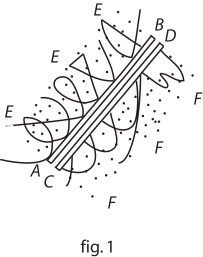
\includegraphics[width=0.33\textwidth]{images/37_3_130r}
%   \\\protect\rule[0cm]{1.5cm}{0cm}\normalsize\textit{[Fig. 2]}
%   %\caption{Bildbeschreibung}
%   \end{wrapfigure}
pour expliquer la \edtext{refraction\protect\index{Sachverzeichnis}{r\'{e}fraction},}{\lemma{refraction}\Bfootnote{\textsc{R. Descartes}, \cite{00038}\textit{La dioptrique}, Leiden 1637, S.~23 (\textit{DO} VI, S.~103).}} sans aucune necessit\'{e} et hors toute l'apparence, peu de gens (hors mis les sectateurs jur\'{e}s) estant satisfaits de ce qu'il a dit sur la refraction\protect\index{Sachverzeichnis}{r\'{e}fraction}, dont les phenomenes je promets d'expliquer mechaniquement, par la seule pression, sans me servir de pores. Cependant ceux qui se plaisent \`{a} nous forger tant de matieres subtiles\protect\index{Sachverzeichnis}{mati\`{e}re!subtile}, ont crû d'avoir trouu\'{e} dans l'Experience de Mons. Hugens\protect\index{Namensregister}{\textso{Huygens} (Hugenius, Vgenius, Hugens, Huguens), Christiaan 1629\textendash 1695}, de quoy confirmer leurs opinions, ayant avanc\'{e} avec confidence, ce que Monsieur Hugens\protect\index{Namensregister}{\textso{Huygens} (Hugenius, Vgenius, Hugens, Huguens), Christiaan 1629\textendash 1695} a propos\'{e} avec tant \edtext{de scrupule, et}{\lemma{tant}\Afootnote{ \textit{ (1) }\ de \textit{ (2) }\ de scrupule, et \textit{ L}}} circumspection digne d'un grand philo\-sophe, accoustum\'{e} plustost \`{a} nous donner des demonstrations que des \edtext{con\-jectures;}{\lemma{conjectures}\Bfootnote{\textsc{Chr. Huygens}, \cite{00062}\textit{Extrait d'une lettre}, \textit{JS} (1672), S.~139 (\textit{HO} VII, S.~205f.).}} s\c{c}avoir une pression d'une matiere\protect\index{Sachverzeichnis}{mati\`{e}re!subtile} plus subtile que l'air, laquelle penetre sans difficult\'{e}, le verre, l'eau et le mercure\protect\index{Sachverzeichnis}{mercure}, et tous les autres corps\protect\index{Sachverzeichnis}{corps} que nous voyons impenetrables \`{a} l'air; et ayant un mouuement en tous sens (selon l'explication de quelques uns) qui frappe \edtext{de deux costez}{\lemma{}\Afootnote{de deux costez \textit{ erg.} \textit{ L}}} les surfaces exterieures de deux corps\protect\index{Sachverzeichnis}{corps} contig\"{u}s, est cause de leur union, aussi bien dans le Recipient \'{e}puis\'{e}, que dans l'air libre. 
Mais cette Hypothese est incommod\'{e}e par les mêmes pores, sur lesquels elle est fond\'{e}e, et les remedes qu'on a apport\'{e}s ne guerissent pas le mal. \edtext{Pour faire comprendre cela parfaitement, supposons dans la \textso{fig 1.} deux corps}{\lemma{mal.}\Afootnote{ \textit{ (1) }\ L'objection est, que supposant des pores dans les corps\protect\index{Sachverzeichnis}{corps|textit} \textit{ (2) }\ Pour [...] corps \textit{ L}}}, \edtext{polis,}{\lemma{}\Afootnote{polis, \textit{ erg.} \textit{ L}}} dont les superficies interieures \textit{AB} et \textit{CD} sont exactement contig\"{u}es, dans une liqueur\protect\index{Sachverzeichnis}{liqueur} ou matiere fluide\protect\index{Sachverzeichnis}{mati\`{e}re!fluide} \textit{EF} \edtext{toute}{\lemma{\textit{EF}}\Afootnote{ \textit{ (1) }\ dans laqu \textit{ (2) }\ toute \textit{ L}}} troubl\'{e}e par une infinit\'{e} de vagues en tous sens